\documentclass[aspectratio=169,11pt]{ctexbeamer}

\usetheme{Madrid}
\usecolortheme{default}
\usefonttheme{professionalfonts}

\usepackage{amsmath}
\usepackage{booktabs}
\usepackage{graphicx}
\usepackage{tabularx}
\usepackage{array}
\usepackage{xcolor}
\usepackage{hyperref}

\graphicspath{{../figures/}}

\definecolor{DoLaBlue}{RGB}{14, 116, 144}
\definecolor{MutedGray}{RGB}{75, 85, 99}
\setbeamercolor{structure}{fg=DoLaBlue}
\setbeamercolor{frametitle}{fg=white,bg=DoLaBlue}
\setbeamercolor{title}{fg=white,bg=DoLaBlue}
\setbeamertemplate{navigation symbols}{}
\setbeamertemplate{footline}[frame number]

\title[DoLa 事实性增强]{基于 DoLa 解码策略的大语言模型事实性增强方法复现与分析}
\subtitle{本机机制实验、HF 复核与官方 LLaMA-7B 复现结果}
\author{自然语言处理课程大作业}
\institute{NLPpre}
\date{\today}

\newcommand{\code}[1]{\texttt{\small #1}}

\begin{document}

\begin{frame}
  \titlepage
\end{frame}

\begin{frame}{汇报结构}
  \tableofcontents
\end{frame}

\section{背景与目标}

\begin{frame}{问题背景：Hallucination}
  \begin{itemize}
    \item 大语言模型可能生成语言流畅但事实错误的答案。
    \item 自回归解码逐 token 最大化局部概率，容易放大高频共现和表面模式。
    \item 更大的模型记忆更多知识，但也更擅长生成“看起来像答案”的文本。
    \item 课程任务关注：不重新训练模型，能否仅通过 decoding 提升 factuality。
  \end{itemize}

  \vspace{0.4em}
  \begin{block}{示例}
    问：澳大利亚首都是哪座城市？\\
    常见错误：Sydney；事实答案：Canberra。
  \end{block}
\end{frame}

\begin{frame}{项目目标与结果定位}
  \begin{columns}[T,onlytextwidth]
    \begin{column}{0.48\textwidth}
      \begin{block}{已完成}
        \begin{itemize}
          \item 本机可运行 DoLa 机制实验
          \item Greedy / Beam / Sampling / DoLa 对比
          \item Layer selection 与 temperature 分析
          \item 官方 LLaMA-7B TruthfulQA-MC 与 FACTOR
          \item 自写 HF official-style TruthfulQA-MC 全量复核
          \item 报告、图表、PPT、讲稿与可运行脚本
        \end{itemize}
      \end{block}
    \end{column}
    \begin{column}{0.48\textwidth}
      \begin{alertblock}{结果边界}
        \begin{itemize}
          \item 本机 17 条实验用于解释机制，不作为 benchmark 主结果
          \item 论文设置对齐以官方 DoLa LLaMA-7B 为主
          \item HF official-style 结果用于复核自写实现偏差
        \end{itemize}
      \end{alertblock}
    \end{column}
  \end{columns}
\end{frame}

\section{DoLa 方法}

\begin{frame}{DoLa 核心思想}
  \begin{itemize}
    \item Transformer 不同层携带的信息不同。
    \item Premature layer 更容易包含表面模式、局部搭配和高频先验。
    \item Mature layer 给出最终语言建模分布，但仍可能受流畅性偏置影响。
    \item DoLa 使用同一模型内部的 layer contrast，不需要额外训练模型。
  \end{itemize}

  \vspace{0.5em}
  \begin{block}{直觉}
    若错误答案在较早层已经很强，而正确答案主要由成熟上下文证据支持，
    则减去 premature layer logits 可以削弱“流畅但错误”的选项。
  \end{block}
\end{frame}

\begin{frame}{数学形式}
  \small
  以下是本项目采用的 layer contrast 简化写法。实际多选评测中，
  每个候选答案按 token-level likelihood 累加评分。

  \vspace{0.3em}
  给定第 $t$ 个位置，第 $l$ 层 hidden state：
  \[
    h_t^l = \mathrm{TransformerLayer}_l(x_{<t})
  \]

  通过语言模型输出头得到 logits：
  \[
    z_t^l = W_{\mathrm{lm}} h_t^l
  \]

  设 mature layer 为 $M$，premature layer 为 $l$：
  \[
    z_t^{\mathrm{DoLa}} = z_t^M - \alpha z_t^l
  \]

  最终解码分布：
  \[
    p_t^{\mathrm{DoLa}} = \mathrm{softmax}(z_t^{\mathrm{DoLa}} / T)
  \]

  \vspace{0.3em}
  其中 $\alpha$ 是对比强度，$T$ 是 temperature；relative-top filtering 用于限制对比作用在高置信候选 token 上。
\end{frame}

\begin{frame}{DoLa Decoding Pipeline}
  \small
  \begin{center}
  \begin{tabular}{c}
    Prompt input \\
    $\downarrow$ \\
    Forward pass with hidden states \\
    $\downarrow$ \\
    Candidate layer logits \quad + \quad Mature layer logits \\
    $\downarrow$ \\
    Select premature layer \\
    $\downarrow$ \\
    $z_{\mathrm{DoLa}} = z_M - \alpha z_l$ \\
    $\downarrow$ \\
    Greedy / Sampling decoding
  \end{tabular}
  \end{center}

  \vspace{0.2em}
  \begin{block}{本项目实现}
    本机脚本使用透明 layer/logits 复现机制流程；
    HuggingFace 入口用 hidden states 和 LM head 计算真实层 logits；
    官方复现实验直接调用 DoLa 仓库的 TruthfulQA-MC 与 FACTOR 评测脚本。
  \end{block}
\end{frame}

\section{实验设置}

\begin{frame}{本机机制实验设置}
  \small
  \begin{columns}[T,onlytextwidth]
    \begin{column}{0.5\textwidth}
      \begin{block}{数据}
        \begin{itemize}
          \item 英文事实问答：6 条
          \item 中文事实问答：6 条
          \item 困难混淆样本：5 条
          \item 共 17 条，多选形式
        \end{itemize}
      \end{block}
    \end{column}
    \begin{column}{0.46\textwidth}
      \begin{block}{方法}
        \begin{itemize}
          \item Greedy Decoding
          \item Beam Search
          \item Sampling
          \item DoLa
        \end{itemize}
      \end{block}
    \end{column}
  \end{columns}

  \vspace{0.2em}
  \begin{block}{固定参数}
    Seed = 42；mature layer = 12；candidate layers = [2, 4, 6, 8, 10]；
    relative top = 0.08；contrast $\alpha$ = 1.0。该设置用于解释机制和生成图表。
  \end{block}
\end{frame}

\begin{frame}{实验环境与证据层级}
  \small
  \begin{table}
    \centering
    \begin{tabular}{>{\raggedright\arraybackslash}p{0.20\textwidth}
      >{\raggedright\arraybackslash}p{0.36\textwidth}
      >{\raggedright\arraybackslash}p{0.34\textwidth}}
      \toprule
      环境 & 硬件/模型 & 用途 \\
      \midrule
      本地 Windows & 无可用 NVIDIA GPU & 运行机制实验、绘图、报告与 PPT 编译 \\
      服务器 & Ubuntu，2$\times$ RTX 3090 24GB，LLaMA-7B & 官方 TruthfulQA-MC、FACTOR 与 HF official-style 复核 \\
      \bottomrule
    \end{tabular}
  \end{table}

  \begin{alertblock}{汇报原则}
    结论强度按证据层级区分：本机结果解释机制；
    3090 服务器 LLaMA-7B 结果作为当前最接近论文设置的复现实验依据。
  \end{alertblock}
\end{frame}

\section{实验结果}

\begin{frame}{本机 Baseline 对比结果}
  \begin{columns}[T,onlytextwidth]
    \begin{column}{0.48\textwidth}
      \begin{table}
        \centering
        \begin{tabular}{lcc}
          \toprule
          Method & Acc. & Truth. \\
          \midrule
          Greedy & 0.706 & 0.706 \\
          Beam Search & 0.706 & 0.706 \\
          Sampling & 0.412 & 0.412 \\
          DoLa & \textbf{0.882} & \textbf{0.882} \\
          \bottomrule
        \end{tabular}
      \end{table}
    \end{column}
    \begin{column}{0.5\textwidth}
      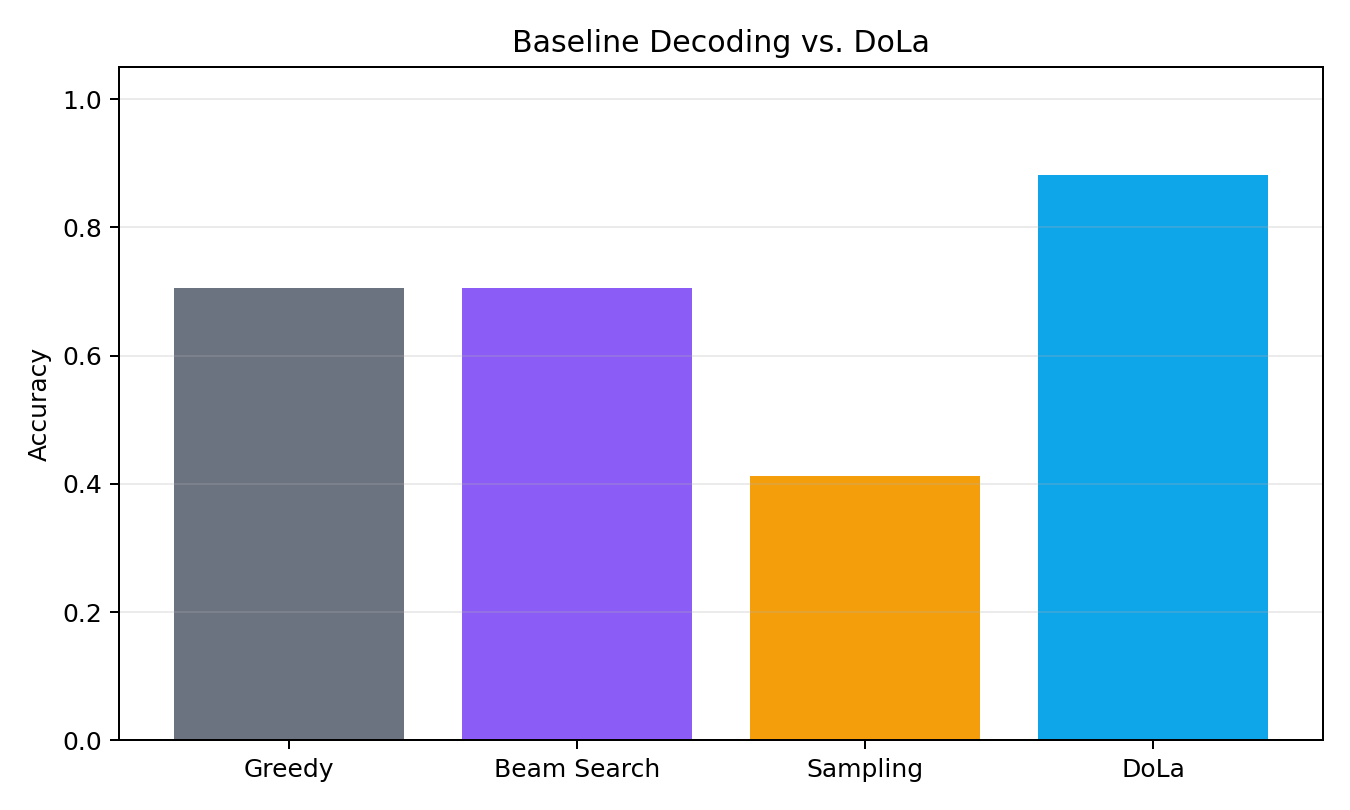
\includegraphics[width=\linewidth]{baseline_vs_dola.png}
    \end{column}
  \end{columns}

  \vspace{0.3em}
  \begin{block}{观察}
    在该 17 条可控样本上，DoLa 比 Greedy/Beam 高 17.6 个百分点；
    Sampling 随机性更强，事实性最低。该结果用于机制说明，不等同于大模型 benchmark。
  \end{block}
\end{frame}

\begin{frame}{官方 LLaMA-7B TruthfulQA-MC 主结果}
  \small
  \begin{table}
    \centering
    \begin{tabular}{lcccc}
      \toprule
      Method & MC1 & MC2 & MC3 & n \\
      \midrule
      baseline & 0.2392 & 0.3925 & 0.1807 & 790 \\
      DoLa high-layer & \textbf{0.3278} & \textbf{0.6540} & \textbf{0.3289} & 790 \\
      \bottomrule
    \end{tabular}
  \end{table}

  \vspace{0.4em}
  \begin{block}{运行条件}
    官方 DoLa 仓库 \code{tfqa\_mc\_eval.py}；模型为 \code{huggyllama/llama-7b}；
    early-exit layers 为 \code{16,18,20,22,24,26,28,30,32}。
    官方脚本最终汇总 790 条可评测样本。
  \end{block}

  \begin{block}{结论}
    DoLa 在 MC1、MC2、MC3 上均高于 baseline，方向与论文主结论一致。
    这里的“高于”指本次复现实验的观测结果，不额外声称统计显著性。
  \end{block}
\end{frame}

\begin{frame}{自写 HF official-style 复核}
  \small
  \begin{table}
    \centering
    \begin{tabular}{lcccc}
      \toprule
      Method & MC1 & MC2 & MC3 & n \\
      \midrule
      vanilla & 0.2392 & 0.3925 & 0.1807 & 790 \\
      DoLa & \textbf{0.3038} & \textbf{0.6445} & \textbf{0.3148} & 790 \\
      \bottomrule
    \end{tabular}
  \end{table}

  \vspace{0.4em}
  \begin{block}{对齐修复}
    使用原始 \code{TruthfulQA.csv} 790 条、官方风格 QA prompt、
    \code{relative\_top=0.0}，并采用 token-level official-like DoLa scoring。
  \end{block}

  \begin{block}{结论}
    vanilla 已与官方 baseline 对齐；DoLa 也明显高于 vanilla。
    与官方 DoLa high-layer 仍有小幅差距，后续主要检查 tokenization、
    early-exit logits 与 \code{lm\_score} 细节。
  \end{block}
\end{frame}

\begin{frame}{官方 LLaMA-7B FACTOR 结果}
  \small
  \begin{table}
    \centering
    \begin{tabular}{llcc}
      \toprule
      Dataset & Method & Accuracy & n \\
      \midrule
      News & baseline & 0.5859 & 1036 \\
      News & DoLa & \textbf{0.6149} & 1036 \\
      Wiki & baseline & 0.5862 & 2994 \\
      Wiki & DoLa & \textbf{0.6219} & 2994 \\
      \bottomrule
    \end{tabular}
  \end{table}

  \vspace{0.4em}
  \begin{block}{运行条件}
    官方 DoLa 仓库 \code{factor\_eval.py}；模型为 \code{huggyllama/llama-7b}；
    early-exit layers 为 \code{0,2,4,6,8,10,12,14,32}。
    News 为 1036 条，Wiki 为 2994 条。
  \end{block}

  \begin{block}{结论}
    DoLa 在 News 和 Wiki 上均高于 baseline，说明在官方 FACTOR 设置下也观察到
    与 TruthfulQA-MC 一致的提升趋势。
  \end{block}
\end{frame}

\begin{frame}{Layer Selection 分析}
  \begin{columns}[T,onlytextwidth]
    \begin{column}{0.48\textwidth}
      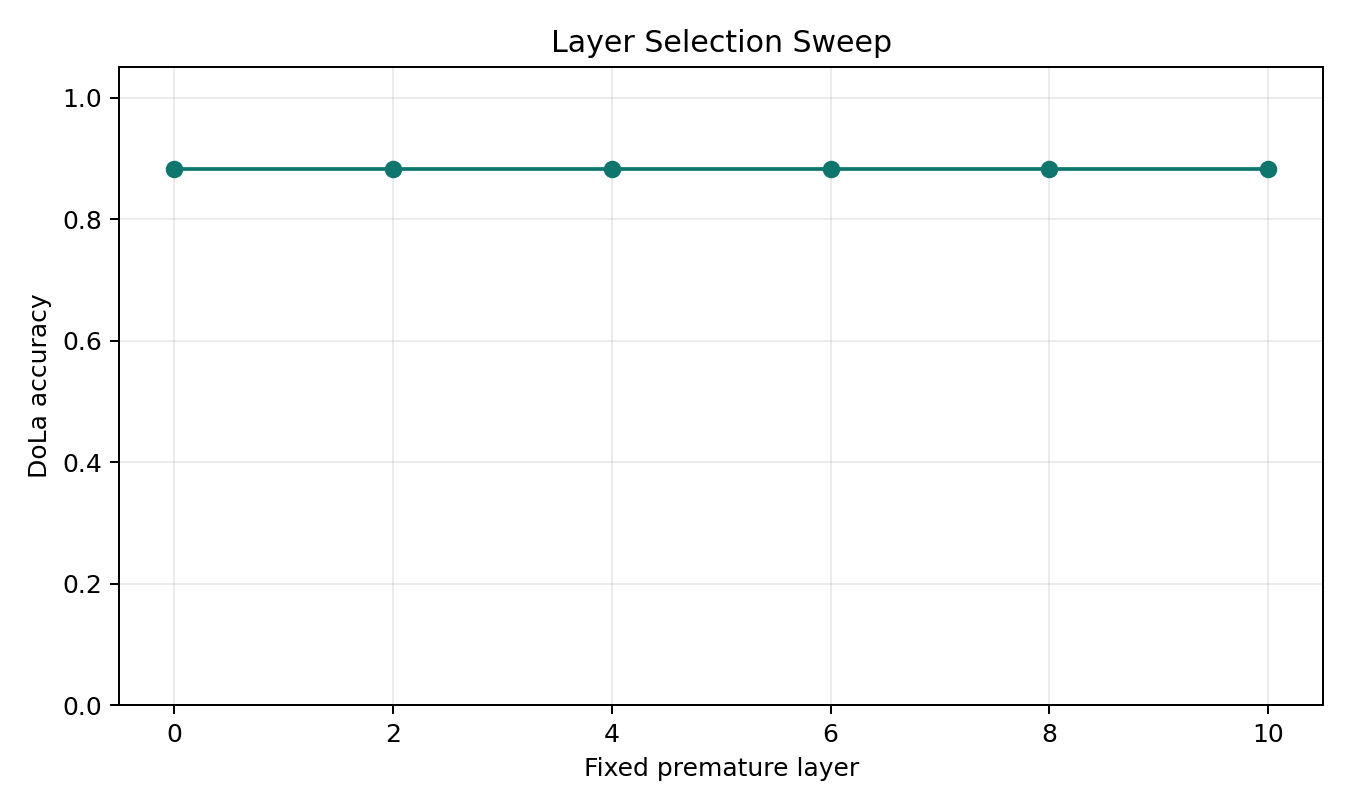
\includegraphics[width=\linewidth]{layer_selection_sweep.png}
    \end{column}
    \begin{column}{0.48\textwidth}
      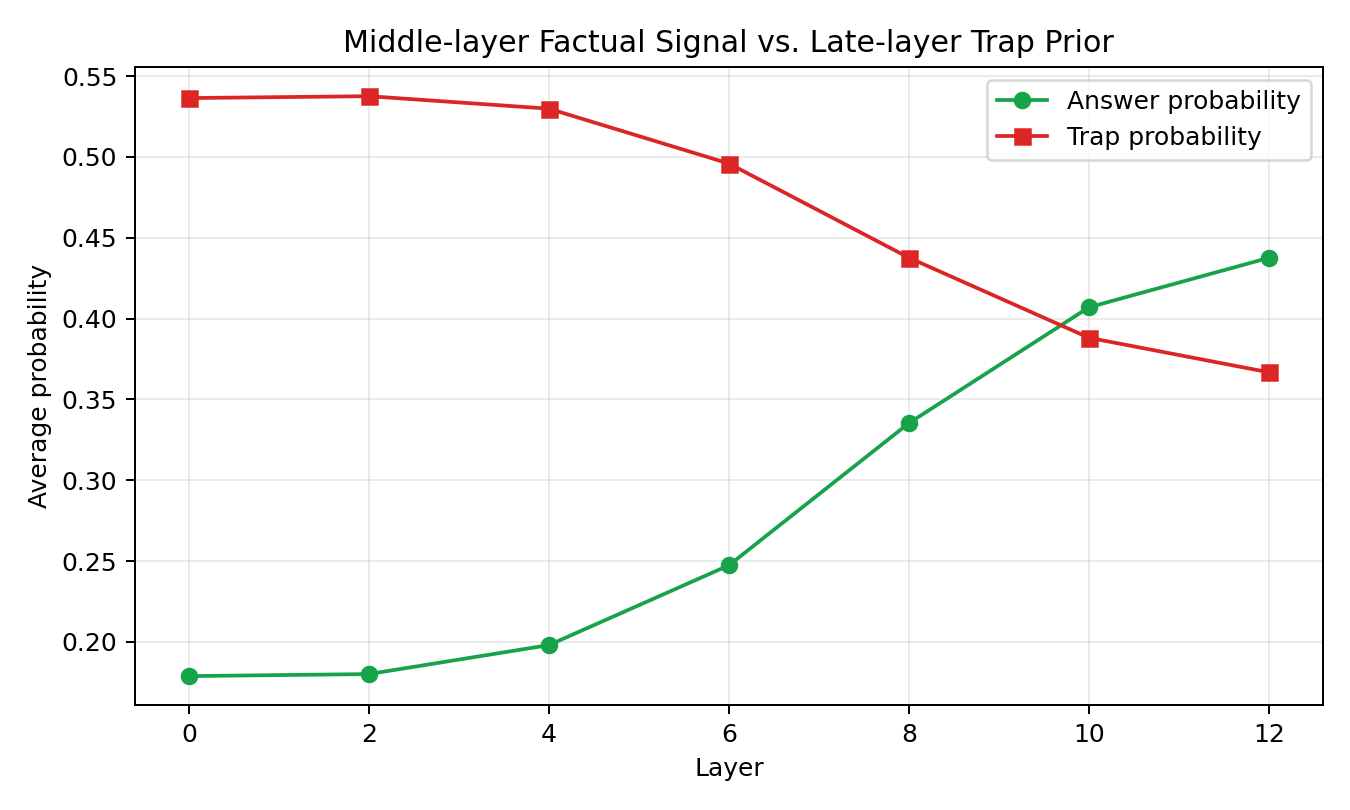
\includegraphics[width=\linewidth]{layer_probability_trace.png}
    \end{column}
  \end{columns}

  \vspace{0.4em}
  \begin{itemize}
    \item 固定不同 premature layer 时，accuracy 在 17 条本机样本上均为 0.882。
    \item 但越接近 mature layer，对比后的 answer probability 越低。
    \item 这提示层间差异变小时，DoLa 可利用的 contrast 信号可能减弱。
  \end{itemize}
\end{frame}

\begin{frame}{Temperature 分析}
  \small
  \begin{columns}[T,onlytextwidth]
    \begin{column}{0.55\textwidth}
      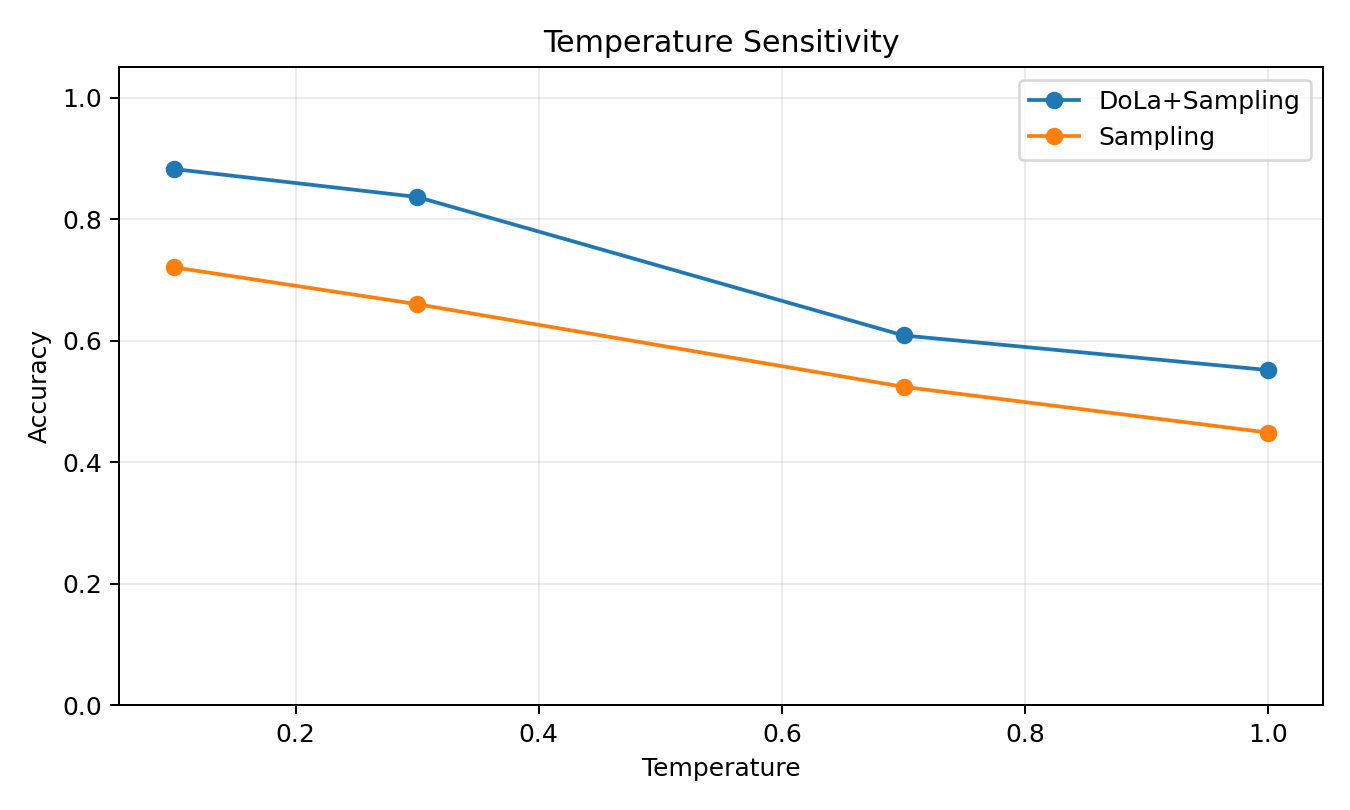
\includegraphics[width=\linewidth]{temperature_sweep.png}
    \end{column}
    \begin{column}{0.42\textwidth}
      \begin{table}
        \centering
        \small
        \begin{tabular}{ccc}
          \toprule
          $T$ & Sampling & DoLa+Sampling \\
          \midrule
          0.1 & 0.721 & \textbf{0.882} \\
          0.3 & 0.660 & \textbf{0.836} \\
          0.7 & 0.524 & \textbf{0.608} \\
          1.0 & 0.449 & \textbf{0.551} \\
          \bottomrule
        \end{tabular}
      \end{table}
    \end{column}
  \end{columns}

  \vspace{0.1em}
  \begin{block}{结论}
    在本机 sampling sweep 中，temperature 升高后 accuracy 整体下降；
    DoLa+Sampling 在四个温度点均高于普通 Sampling。
  \end{block}
\end{frame}

\section{案例分析}

\begin{frame}{DoLa 成功案例}
  \small
  \begin{tabularx}{\textwidth}{>{\raggedright\arraybackslash}p{0.24\textwidth}
    >{\raggedright\arraybackslash}p{0.14\textwidth}
    >{\raggedright\arraybackslash}p{0.14\textwidth}
    >{\raggedright\arraybackslash}X}
    \toprule
    问题类型 & Greedy & DoLa & 分析 \\
    \midrule
    1893 world's fair & Paris & Chicago & Paris 有世界博览会强先验，但题目中的 1893 和 electric lighting 指向 Chicago。 \\
    Chemical symbol W & Tin & Tungsten & W 与英文名 Tungsten 表面不匹配，baseline 偏向更直观的金属名。 \\
    Cobalamin & Vitamin C & Vitamin B12 & Vitamin C 更高频，但 cobalamin 的事实答案是 B12。 \\
    \bottomrule
  \end{tabularx}

  \vspace{0.6em}
  \begin{block}{共同点}
    这些本机案例中，Baseline 错误多来自高频实体、表面联想或常见事实模板；
    DoLa 通过扣除 premature layer 中的陷阱先验修正答案。
  \end{block}
\end{frame}

\begin{frame}{DoLa 失败案例}
  \small
  \begin{tabularx}{\textwidth}{>{\raggedright\arraybackslash}p{0.28\textwidth}
    >{\raggedright\arraybackslash}p{0.16\textwidth}
    >{\raggedright\arraybackslash}p{0.16\textwidth}
    >{\raggedright\arraybackslash}X}
    \toprule
    问题 & 正确答案 & DoLa 输出 & 失败原因 \\
    \midrule
    Who introduced the word ``cell'' after observing cork? & Robert Hooke & Anton van Leeuwenhoek & 两者都与显微镜强相关，属于同一事实邻域内混淆。 \\
    Which country has Sucre as its constitutional capital? & Bolivia & Peru & 需要具体地理政治知识；若模型内部证据弱，DoLa 不能补知识。 \\
    \bottomrule
  \end{tabularx}

  \vspace{0.6em}
  \begin{alertblock}{边界}
    DoLa 是重排模型内部预测分布的方法，不是检索系统。模型不知道或强混淆的事实，仍需要 RAG、验证器或外部知识。
  \end{alertblock}
\end{frame}

\section{结论与后续}

\begin{frame}{结论}
  \begin{itemize}
    \item DoLa 通过同一模型内部的 layer contrast 改变 decoding 分布。
    \item 本机机制实验中，DoLa 的 accuracy/truthfulness 从 0.706 提升到 0.882。
    \item 官方 LLaMA-7B TruthfulQA-MC 中，DoLa 在 MC1/MC2/MC3 上均优于 baseline。
    \item HF official-style 复核中，vanilla 与官方 baseline 对齐，DoLa 明显高于 vanilla。
    \item 官方 LLaMA-7B FACTOR 中，DoLa 在 News/Wiki accuracy 上均优于 baseline。
    \item 本机 temperature 分析显示：更高采样温度会降低 accuracy，DoLa 可部分缓解。
    \item 失败案例说明：DoLa 不能创造模型没有掌握的事实知识。
  \end{itemize}

  \vspace{0.5em}
  \begin{block}{一句话总结}
    DoLa 的价值在于低成本抑制部分“流畅但错误”的生成倾向，但它不是 factuality 问题的完整解法。
  \end{block}
\end{frame}

\begin{frame}{下一步提升方向}
  \begin{enumerate}
    \item 分析 HF official-style 与官方 DoLa 的残余差异：tokenization、early-exit logits、\code{lm\_score}。
    \item 加强 logits 可视化：成功/失败样例的 answer/trap logits 与选层曲线。
    \item 扩展中文事实性数据集，覆盖历史、地理、文学和科学常识。
    \item 增加效率分析：latency、tokens/s、显存、candidate layers 数量影响。
    \item 与 RAG、CoT、self-consistency 等方法做扩展对比。
  \end{enumerate}
\end{frame}

\begin{frame}{代码与输出}
  \scriptsize
  \begin{itemize}
    \item 本机实验：\code{scripts/run\_local\_dola\_demo.py}
    \item 真实模型入口：\code{scripts/run\_hf\_mc\_eval.py}
    \item 官方 TruthfulQA：\code{scripts/run\_official\_dola\_truthfulqa.sh}
    \item 官方 FACTOR：\code{scripts/run\_official\_dola\_factor.sh}
    \item 实验结果：\code{outputs/local\_results\_summary.csv}
    \item 官方 TruthfulQA 结果：\code{outputs/official\_dola\_truthfulqa\_summary.csv}
    \item HF official-style 结果：\code{outputs/hf\_official\_fix/llama7b\_official\_style\_full\_summary.csv}
    \item 官方 FACTOR 结果：\code{outputs/official\_dola\_factor/factor\_summary.csv}
    \item 案例分析：\code{outputs/case\_studies.csv}
    \item 图表目录：\code{figures/}
    \item 报告：\code{report/report.md}
  \end{itemize}

  \vspace{0.2em}
  \begin{block}{参考}
    DoLa: Decoding by Contrasting Layers Improves Factuality in Large Language Models, ICLR 2024.\\
    \url{https://openreview.net/forum?id=Th6NyL07na}
  \end{block}
\end{frame}

\begin{frame}
  \centering
  \Huge 谢谢
\end{frame}

\end{document}
